\chapter{THE STANDARD MODEL} \label{sm}

The Standard Model (SM) of particle physics is an incredibly successful theory that correctly describes the physics of all known particles and forces that make up the universe, excluding gravity \cite{smconsistency}. The particles of the SM come in two types, fermions and bosons \footnote{Bosons have integer spin.}. Fermions are the spin 1/2 particles and make up the different types of matter. Electrons are a familiar example, and the up and down quarks that make up protons and neutrons are some other examples of fermions. While electrons and the up and down quarks account for nearly all of the matter in our day to day experience there are actually many other fermions. In fact, there are three generations of quarks and leptons \footnote{Leptons are fermions that aren't quarks.} with each generation heavier than the next. The up and down quarks are the first generation of quarks, charmed and strange are the next, and top and bottom are the third generation. For the leptons the electron and electron neutrino are the first generation, the muon and muon neutrino are the second, and the tau and the tau neutrino the third. Each fermion also has a corresponding antiparticle. As an example, the positron is the antiparticle for the electron. 

\begin{figure}[h!]
  \centering
  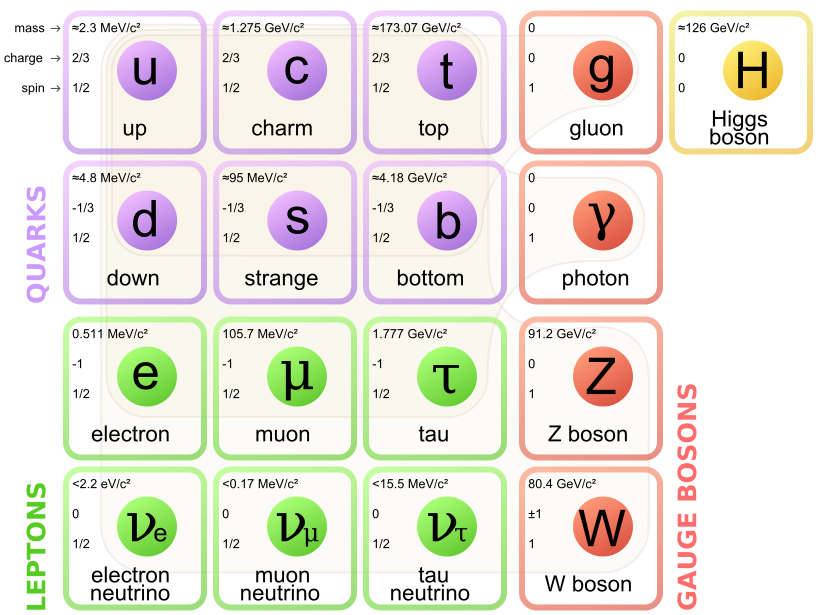
\includegraphics[width=4in]{images/Standard_Model_of_Elementary_Particles.png}
  \caption
   {The Standard Model Particles}
  \label{fig:smtable}
\end{figure}

The universe would be pretty boring if the particles couldn't attract or repel or form more complex objects like atoms, molecules, and even people. Luckily there are forces as well and these forces are described by the spin 1 bosons. The fermions attract and repel by exchanging bosons, which is why the bosons are often called force carriers. Gluons mediate the strong force, photons the electromagnetic force, and the W and Z bosons mediate the weak force. Every force has an associated charge. Just as those particles with electric charge can interact through the electromagnetic force, those with color charge may interact via the strong force, and those with isospin may interact through the weak force. The fundamental forces and particles interact to make the familiar composite objects that surround us in our daily lives. The strong force binds quarks to form protons and neutrons, the Van Der Waals version of the strong force binds the protons and neutrons together to form nuclei, and the electromagnetic force binds electrons and nuclei to form atoms. The size of the composite objects gives an idea of the relative strength of the forces. A proton is ~$10^-15$ meters in size while an atom is ~$10^-10$ meters and a solar system is ~$10^12$ meters. The more tightly bound the stronger the force. In fact the ratio of the strength of the forces is like so 1:$10^-3$:$10^-16$:$10^-41$, strong : electromagnetic : weak :gravitational \footnote{Gravity is just included for perspective. The Standard Model does not describe this force and reconciling gravity with quantum mechanics is an open problem.}. 

Of all the particles predicted by the SM, only the Higgs boson remains to be found. The Higgs boson is the only spin 0 particle of the SM. It is theorized that as the universe cooled from the Big Bang the Higgs field went through a phase transition and settled into a nonzero ground state forming a condensate. And it is the potential energy from the interactions with this ground state that give the massive fundamental particles their mass. With such a large role in the SM, finding this particle or a BSM Higgs has been a huge priority for the CMS collaboration \cite{tdr}. In 2012 a Higgs particle with a mass of 125 GeV was found and to date remains consistent with the Standard Model. However, the properties need to be investigated further before declaring the discovered Higgs the Higgs of the Standard Model. 


%%%%%%%%%%%%%%%%%%%%%%%%%%%%%%%%%%%%%%%%%%%%%%%%%%%%%%%%%%%%%%%%%%%%%%%%%%%

\section{Quantum Field Theory}

The mathematical framework used to describe the physics of the SM as well as other Beyond Standard Model (BSM) field theories is called Quantum Field Theory (QFT). QFT enables the predictions of measurable quantities, namely the probabilities for different sets of particles to come out of a specific collision or for a single particle to decay into different sets of particles. These probabilities are encompassed in the cross sections and branching fractions. For example, the theory of the SM predicts the cross section for two protons colliding and making a Higgs. As another example, the SM also predicts the branching fraction for a Z boson decaying to two muons. These probabilities can be measured simply by colliding particles and counting the outcomes which in turn means that the theory can be tested. In fact, any QFT model can be tested in this manner. There are other commonly measured properties as well like the lifetime, spin, and mass of different particles.  

\subsection{What is a Particle?}

\subsection{QFT From Symmetry}

\subsection{Perturbation Theory}

\subsection{Feynman Rules}

\begin{figure}[h!]
  \centering
  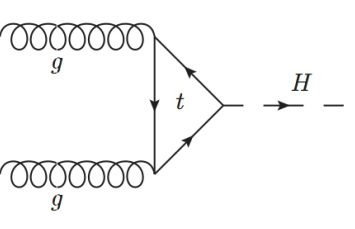
\includegraphics[width=1.5in]{images/ggf.png}
  \caption
   {The Feynman diagram for two gluons fusing into a Higgs. There are three vertices and this is a third order diagram. Two vertices involve the strong force and one vertex involves the Higgs coupling. The matrix element for this diagram would have two factors of the strong force coupling and one factor for the Higgs coupling which involves the mass of the top quark.}
  \label{fig:feynggf}
\end{figure}

%%%%%%%%%%%%%%%%%%%%%%%%%%%%%%%%%%%%%%%%%%%%%%%%%%%%%%%%%%%%%%%%%%%%%%%%%%%
\section{The Standard Model Higgs}


%%%%%%%%%%%%%%%%%%%%%%%%%%%%%%%%%%%%%%%%%%%%%%%%%%%%%%%%%%%%%%%%%%%%%%%%%%%
\subsection{SM Higgs Production and Decay Modes}

The SM Higgs can be created in a variety of ways. Some of these cross sections are shown below for 14 TeV collisions. The production cross sections are functions of the mass of the Higgs as well as the energy of the collisons. For a given collision energy the cross sections decrease as the Higgs mass increases: there are fewer kinematic possibilities for a heavier particle since more of the energy was used to create the particle. For a given mass, say 125 GeV, the cross section grows with collision energy. This constrasts with cross sections involving collisions of fundamental particles, e.g. electron antielectron collisions. This is an artifact of the fact that the LHC collides protons together. 

\begin{figure}[h!]
  \centering
  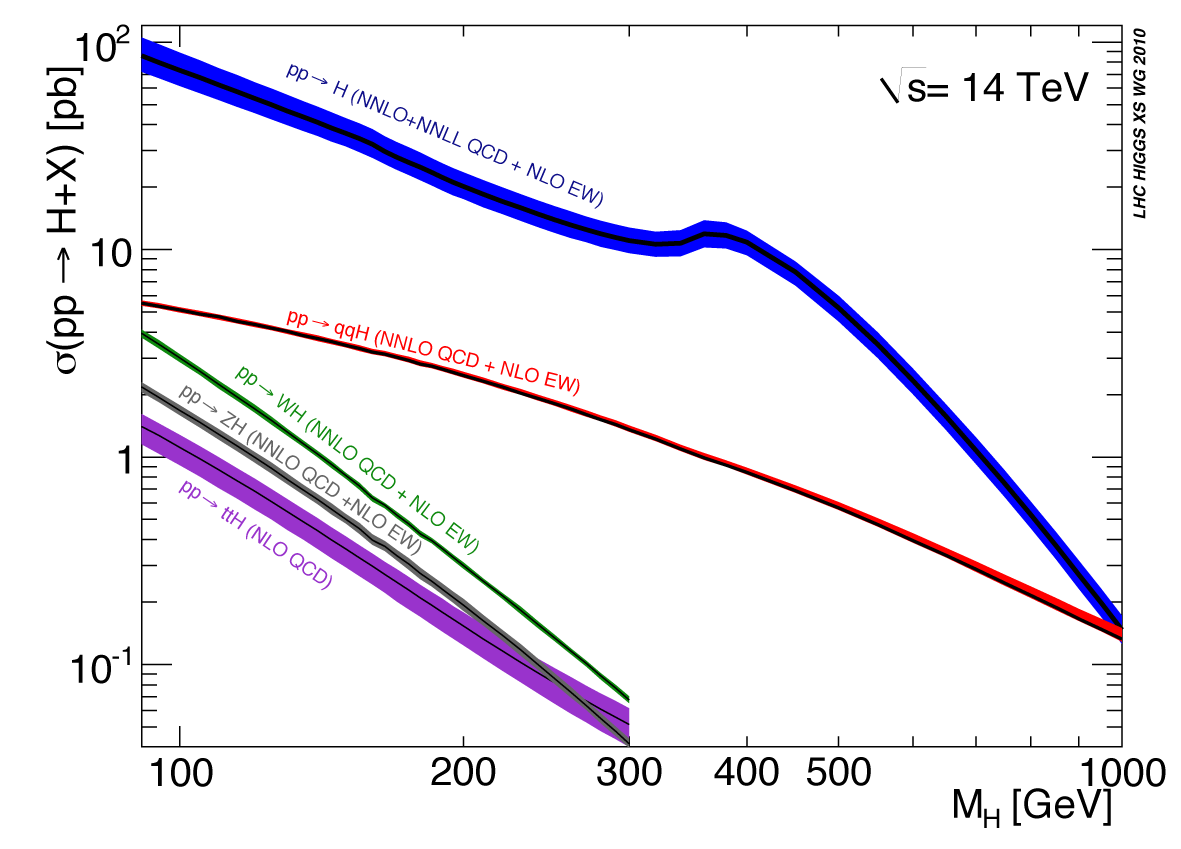
\includegraphics[width=5in]{images/14TeV_higgs_cross_sections.png}
  \caption
   {The highest production mode cross sections for the SM Higgs \cite{crossbranchplots}}
  \label{fig:hprodcross}
\end{figure}

Protons behave like a collection of an infinite number of quark-antiquarks, an infinite number of gluons, and the usual uud. The total momentum of the proton is divided up amongst them with lots of particles having little of the total momentum. The actual scattering events are between these more fundamental particles. The larger the total energy the smaller the fraction of energy needed to make a Higgs and since there are more particles with a lower fraction, this results in a growth of the cross section with collision energy. 

The SM Higgs is unstable and decays with a width of $\sim 5 MeV$ at 125 GeV. The probability of each decay changes depending upon the mass of the Higgs. In general the Higgs couples more strongly to particles with higher mass making the decays to heavier particles more likely.  

\begin{figure}[h!]
  \centering
  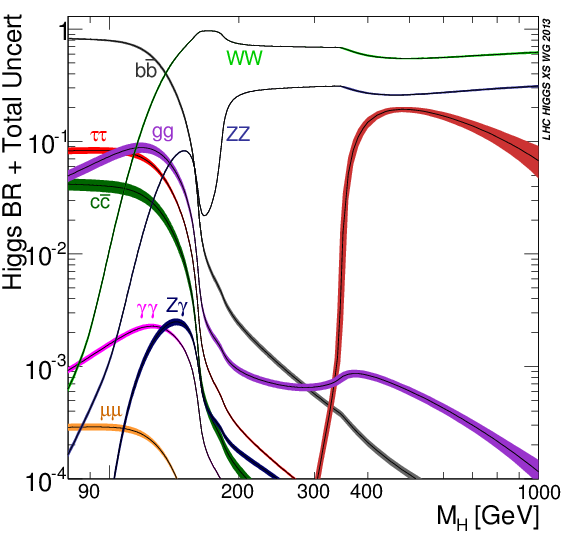
\includegraphics[width=3in]{images/Higgs_BR.png}
  \begin{tabular}{ |l|l| }
    \hline
    \multicolumn{2}{|c|}{Higgs Branching Ratios} \\
    \hline
    ${\rm b\bar{b}}$ & 0.57 \\
    WW & 0.22\\
    gg & 0.085 \\
    ${\rm \tau\tau}$ & 0.065 \\
    ZZ & 0.027 \\
    ${\rm c\bar{c}}$ & 0.027 \\
    ${\rm \gamma\gamma}$ & 0.0023 \\
    ${\rm Z}\gamma$ & 0.0016 \\
    ${\rm \mu^{+}\mu^{-}}$ & 0.00022 \\
    \hline
  \end{tabular} 
  \caption
{The graphic on the top left presents the SM Higgs branching fractions as functions of mass while the table on the bottom right displays the branching fractions for a 125 GeV SM Higgs \cite{crossbranchplots}.}
  \label{fig:hbranch}
\end{figure}

The muon has the lowest mass -- excluding the photon and gluon -- of the particles in Figure ~\ref{fig:hbranch} and consequently H$\rightarrow \mu^{+}\mu^{-}$ has the lowest branching fraction in the set. \footnote{The Higgs also couples to the electron and the first generation quarks but the masses are so light that CMS does not expect to see the SM Higgs in those modes.} The gluons and photons are massless and do not couple to the Higgs at leading order. These massless vector bosons interact with the Higgs through a loop of top quarks. The extremely heavy mass of the top quark, about 173 GeV, balances the fact that the loop production is a higher order mechanism.  
\begin{figure}[h!]
  \centering
  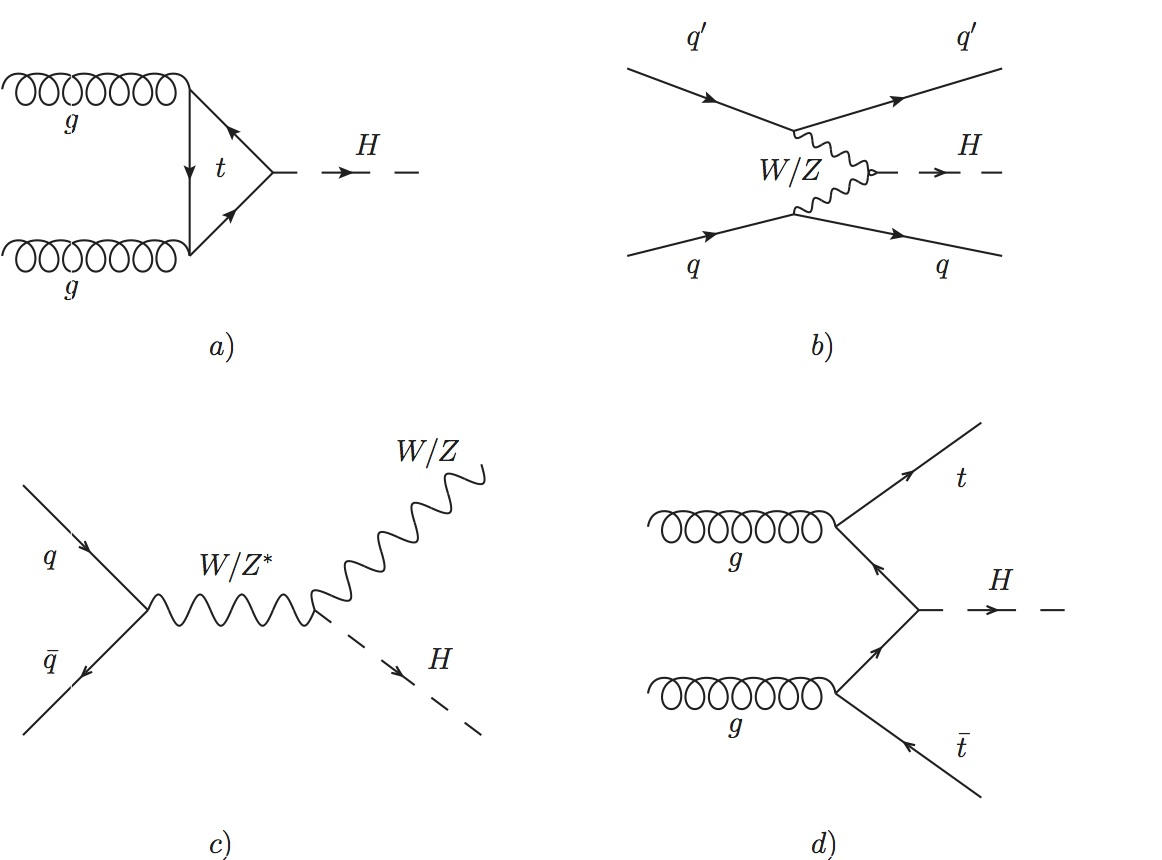
\includegraphics[width=4in]{images/higgs_production_modes.png}
  \caption
   {The SM production modes with the highest cross sections. a) Gluon Gluon Fusion (GF) b) Vector Boson Fusion (VBF) c) Associated Production with a Vector Boson (VH) d) ${\rm t\bar{t}}$H}
  \label{fig:hfeynprod}
\end{figure}

The Higgs to massless vector boson coupling via the top loop is seen in the GF Feynman diagram in Figure ~\ref{fig:hfeynprod}. At ${\rm M_{h} = 125}$ GeV, ${\rm \sqrt{s} =}$ 13 TeV, the GF channel comprises 87\% of the total Higgs production cross section, VBF 7\%, VH 4\%, and ${\rm t\bar{t}}$H 1\% \cite{crossbranchplots}. Besides ${\rm t\bar{t}}$H, the process q + $\bar{q} \rightarrow$ H isn't considered due to its low cross section. The low masses of the other quarks suppress the process. 

Quark gluon (qg) scattering is a major background for the Higgs to two jets decays since the process closely resembles GF in this mode.   

\begin{figure}[h!]
  \centering
  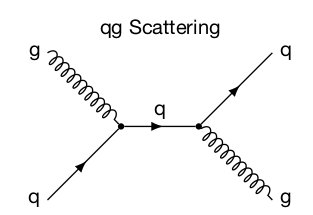
\includegraphics[width=2in]{images/qg_scattering.png}
  \caption
   {Quark gluon scattering creates many two jet events. This background looks very similar to GF when the Higgs decays to two jets. The colliding protons are made of quarks and gluons so this process is extremely common.}
  \label{fig:feynqg}
\end{figure}

